\chapter{Overview}

    There are diverse SDN controllers accessible. Some of them are open source ventures created and kept up by the network, while private associations build up a few. Notwithstanding open source or private, all controllers follow a similar rule of equipment autonomy and the partition and overcome approach. Similarly, as with any situation where there are numerous choices of a certain something, a decision is made in light of the fact that we can't send all the alternatives in a similar domain at the same time.
 
    To choose the best controller, first, there is a need to comprehend the idea of the best controller. What are the standards on which controllers should be judged or analysed? Is there even a potential best controller among them all. Like how we measure separation utilising a ruler, or time using a clock, we need a standard against which controllers can be thought about, and afterwards contrast the examinations and one another. This standard of measurements is urgent to choosing which controller would be perfect. There are a few papers which notice a couple of essential measurements, let us investigate.
    
   Controllers must be analyzed on a few models. Past papers talked about a wide assortment of properties of controllers going from physical execution to adaptation to internal failure. A portion of the measurements incorporate time for setting up the system, tearing down the system, preparing power Usage, potential to scale the system, CPU use, memory use, throughput, latency, ping delay, etc.
    
     On an industrial level, these above metrics clearly gave an idea of the controller's performance. Nevertheless, these all criterion seems very well researched and are also evolving with coming hardwares and new features in the tools and controllers. Factors like system utilization also have to be evaluated to determine whether the controller uses the hardware constraints efficiently. It also gives a clear idea about the controller's nature while it is running and helps identify the system bottlenecks.
    
    A paper published in 2018 came up with methodologies for measuring the performance of all controller implementations and benchmarked the control- plane performance \cite{rfc8456}.
    
    Another paper, published in 2019, describes some repeated tests by using a benchmarking tool and a network emulator that included the CPU utilization of various Controllers on a machine. It uses a benchmark tool which operates on a different system, that sends a considerable amount of random packets to the controller and then reads CPU utilization values. Fig. \ref{figzhu2019sdn} below depicts the average CPU utilization at a given time. The diagram gets populated by information from the benchmarking tool, which plays out the test consistently. In this, a virtual machine is used to run the controller operating system \cite{zhu2019sdn}. Currently, the benchmark OFNet used in that experiment is no longer available as the concerned owner has removed it.
    
    A paper, published in 2014, describes how OFCBench and OFCProbe can be used as CPU and RAM utilization monitor and find bottlenecks of the controller. The implementation of these monitors is by sending SMTP messages from client machines. However, it is worth noting that both these tools are limited to work with Floodlight, Ryu, and Nox Controllers. \cite{ofcprobe}
    
    One more paper, published in 2012, shows they used multiple instances of CBench to send packets and measure the CPU Utilization. They discovered an inherent performance bottleneck concerning CPU load in OpenFlow switch implementations of those days. \cite{flexible}
    
\begin{figure}[!hbt]
    \centering
        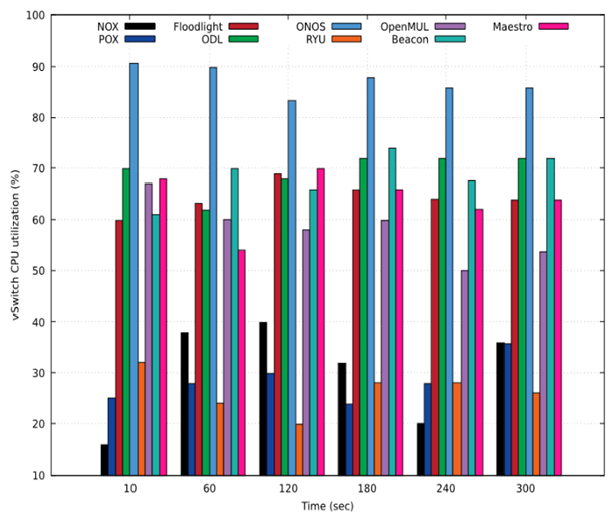
\includegraphics[width=\textwidth,keepaspectratio]{images/zhucpu.png}
       \caption{CPU Utilization Results Published \cite{zhu2019sdn}}
        \label{figzhu2019sdn}
\end{figure}

   The throughput method of CBench in which the switches are arranged to pause and heap up a lot of packets and send all the packets without a moment's delay to the controller. This powers the controller to dispense a huge portion of its resources to each or two switches in turn. This method gauges the pressure limit of the controller. The controller must have enough memory to store and procedure all the solicitations from a switch. It need not have the option to run such a large number of strings simultaneously.

        The tests acted in the paper \cite{dynamicrouting} think about numerous controllers, running in a system whose size increments. For this component, they expanded the number of hubs after each arrangement of tests and rehashed them while recording the outcomes. What appears to be neglected in this test is that the outcomes are legitimate, furnish us just with a fundamental thought of the controller's performance. The controller with the best development of the response rate in relation to organizing size was delegated the best controller.
        
    The controller gives more reactions as the network size increment. It is on the grounds that there is more packets in occasions from switches. As the network size builds, more courses should be determined and kept up. More changes should be refreshed normally. Nonetheless, one factor is ignored. The way that more requests are created isn't really on the grounds that there are more switches; it is on the grounds that there are more has in general associated with the network. The trial proceeded as in paper \cite{routingtie2017} by expanding the number of switches while keeping up the number of hosts per switch. As the network grows, more has would need to impart, in this way promoting the ascent in route requests or packets in occasions.
    
    \textit{Traffic Intensity} is a measurement technique to test floodibility of a network's traffic. As the network gets scaled up, the number of hosts increases, thus increasing traffic Intensity. This expansion in network traffic intensity powers the controller to expand its exhibition rates to adapt to the network necessities. There is a requirement for a strategy to think about the controller with the end goal that base outside elements are impacting the controller's performance. In the experiment, the traffic intensity is kept very high to perceive how various controllers handle the situation and how their performance is influenced.

    For any test, nature inside which the subject to be tried must be separated from outer factors however much as could be expected. So in the experiment, the cores of CPU where the controller runs, needs to be isolated using \textit{isolcpus} or similar tool.